\documentclass[10pt,a4paper,notitlepage]{article}
\usepackage[latin1]{inputenc}
\usepackage{amsmath}
\usepackage{amsfonts}
\usepackage{amssymb}
\usepackage{graphicx}
\usepackage[procnames]{listings}
\usepackage{color}
\usepackage{caption}
\usepackage{subcaption}
\author{S. Bechan(4146425), K. Elgin(4163389), Z. Ramlakhan(4170229)}
\title{MD}
\begin{document}

    \maketitle
    \begin{center}
    \line(1,0){350}
    \end{center}
    \begin{abstract}
      As part of the International Course Computational Physics of the Master Applied Physics program, students are required to simulate the molecular dynamics of Argon molecules. In this report the movement and the interactions of these molecules are simulated in a box. Simulations were based on Verlet's algorithms, which provides iterative methods to determine the positions and velocities of the particles. From these quantities parameters such as the specific heat, pressure and the pair correlation were calculated and plotted. 
 
    \end{abstract}
    \begin{center}
    \line(1,0){350}
    \end{center}

\section{Introduction}\label{sec:intro}
Molecular dynamics (MD) is a field of study which uses computer simulatios to depict the movement and interactions of a number of particles confined to a box. The trajectories of the particles are determined by numerically solving Newton's equations of motion. The potential energy $U(r)$ of each particle is given by the \textit{Lennard-Jones potential}, also known as the 6-12 potential,

\begin{equation}\label{LJ}
U (r)= 4\epsilon\left[\left(\frac{\sigma}{r}\right)^{12} - \left(\frac{\sigma}{r}\right)^6\right]
\end{equation}

with the $\epsilon$ the depth of the potential well and $r$ the distance between two particles. It is evident then that $\sigma$ represents the distance between two particles such that $U(\sigma)=0$.\\
The force $\textbf{F}$ the particles exert on each other is given by

\begin{equation}\label{F}
\textbf{F}= -\nabla  U(r)
\end{equation}

The simulation's algorithm consists of a few steps. First the particles are given an initial position and a time step is defined. The forces the particles exert on each other are then calculated from which the acceleration can also be found. The equations of motion yield the new position as well as velocity of the particles. At this point time is moved forward with the time step. The forces are calculated again and the process repeats itself for a desirable number of iterations. This method is called the Verlet algorithm.\\

The following is a report of MD simulation of argon gas in the low temperature limit. The report in particular elaborates on translation of the physical formulas to a code and explaining the steps taken.

\section{Simulation}\label{sec:sim}
Section \ref{sec:intro} described the MD algorithm. This section will explain in more detail how to get from physical formulas to a MD simulation code.
\subsection{Initial position}\label{sec:init_pos}
Argon particles are subjected to a face-centered cubic (FCC) lattice which means there are four lattice points per unit cell. The initial positions of $n$ particles can be generated by first defining a unit cell with Cartesian coordinates $(0,0,0),(0.5,0.5,0),(0.5,0,0.5),(0,0.5,0.5)$. Other unit cells are then "stacked" on top of the first cell in the $x,y,z$-directions such that $n$ is equal to four times the number of stacked cells in a single direction raised to the power three.\\
The system of particles has a total volume $V$ of 

\begin{equation*}
V = \frac{nm}{\rho} = \frac{n}{\rho} = L^3 \Leftrightarrow L = \left(\frac{n}{\rho}\right)^{\frac{1}{3}}
\end{equation*}

with the particle mass $m$ and density $\rho$. $m$ is set to 1 to reduce computational effort. Taking the cubic root of $V$ results in the dimension of the box $L$ which confines the particles. The result is an array describing the initial positions of $n$ particles in a fcc lattice confined to a box of dimension $L$.

\subsection{Initial velocity}\label{sec:init_vel}
The particle speed $v$ is defined by the Maxwell-Boltzmann distribution

\begin{align}\label{MBD}
f(v) &= \sqrt{\left(\frac{m}{2\pi k_B T}\right)^3}4\pi v^2 e^{-\frac{mv^2}{2k_BT}} \nonumber\\
	 &= \sqrt{\left(\frac{1}{2\pi T}\right)^3}4\pi v^2 e^{-\frac{v^2}{2T}}
\end{align}
 
 with the Boltzmann constant $k_B$  and the temperature $T$. Like $m$, $k_B$ is also set to 1. To generate the random speeds of the particles the cumulative distribution function $CDF$ is calculated for a range of speeds. $CDF$ is given by the integral over $f(v)$ from $-\infty$ to $v$, the result of which is 
 
 \begin{equation}\label{cdf}
 CDF = erf\left(\frac{v}{\sqrt{2T}}\right) - \sqrt{\frac{2}{\pi}}v e^{-\frac{v^2}{2T}}
 \end{equation}
  
  $CDF$ is defined over the range $[0,1]$, so by generating a random number from that range and interpolating it against $CDF$ yields a particle random speed.\\
  The speeds are given a direction by multiplying them with random spherical coordinates which translates the velocity vectors to Cartesian coordinates.
  
  \subsection{Force}
  The potential $U(r)$ was already given in \eqref{LJ}. $\sigma$ and $\epsilon$ are set to 1 as well. Furthermore, $U(r)$ can be represented as the sum of pairwise interactions
  
  \begin{align}\label{LJ_ij}
  U(r) &=\displaystyle\sum^n_{i=1}\displaystyle\sum^n_{i<j}u(r_{ij})  \nonumber\\
       &=\displaystyle\sum^n_{i=1}\displaystyle\sum^n_{i<j}4\left(\frac{1}{r^{12}_{ij}} - \frac{1}{r^6_{ij}}\right)
  \end{align}
  
  with $r_{ij}$ the magnitude of the vector \boldmath{$r_{ij} = r_i -r_j$}.\unboldmath The total force working on particle $i$ is given by taking the negative gradient of \eqref{LJ_ij},
  
  \begin{align}\label{F_i}
  \textbf{F}_i &= \displaystyle\sum^n_{i\neq j} \textbf{f}_{ij} = \displaystyle\sum^n_{i\neq j} - \frac{du(r_{ij})}{dr_{ij}} \cdot \frac{\textbf{r}_{ij}}{r_{ij}}\nonumber\\
   &=\displaystyle\sum^n_{i\neq j} -24\left(  \frac{2}{r^7_{ij}}-\frac{1}{r^4_{ij}}\right) \cdot \textbf{r}_{ij}
  \end{align}

\subsection{Iteration}
The positions and velocities of the particles are updated every iteration and are done so by obeying the equations of motion. Suppose $r(t),\textbf{v}(t)$ represent the initial position and velocity of a particle, respectively. Then $r(t+\Delta t),\textbf{v}(t+\Delta t)$ represent that particle's position and velocity after one iteration. The relations between these quantities are given by
\begin{align}
\textbf{v}(t+\Delta t) &= \textbf{v}(t) + \textbf{a}(t)\Delta t\nonumber\\
                       &= \textbf{v}(t) + \textbf{F}(t)\Delta t\\\label{v_iter}
r(t+\Delta t)          &= r(t) + \textbf{v}(t)\Delta t + \frac{1}{2}\textbf{a}(t)\Delta t^2\nonumber\\
                       &= r(t) + \textbf{v}(t)\Delta t + \frac{1}{2}\textbf{F}(t)\Delta t^2 
\end{align}
This method is called the Verlet algorithm.
\section{Physical parameters}\label{sec:phys}
From the simulation a number of physical parameters can be calculated.
\begin{itemize}
\item The total energy $E_t$ is given by the sum of the potential, given by \eqref{LJ_ij}, and the kinetic energy of all particles and is a conserved parameter. The kinetic energy of the system is given by 

\begin{equation}\label{Ek}
E_k = \frac{1}{2}\displaystyle\sum^n_{i=1}\textbf{v}^2_i 
\end{equation}
Via the equipartition theorem, $E_k = \frac{3}{2}k_BNT$, the relation between the velocity of the particles and the temperature of the system becomes clear i.e.
\begin{equation}\label{T}
T = \frac{2k_BE_k}{3n}
\end{equation}
\item The pair correlation function (or radial distribution function)

\begin{equation}\label{g}
g(r) = 4\pi r^2_{ij} \frac{n}{V}dr
\end{equation} 
represents the probability of two particles being separated a distance $r$. Due to repulsive forces, there is a minimal distance the particles can be separated from each other. On the other hand, attractive forces prevent the particles from getting to far from each other. \eqref{g} therefore shows the range of possible separation distances and the probability of those separation distances.

\item The pressure can be derived from the virial theorem which, for a pair potential, is given by
\begin{equation}\label{vir}
PV =  nk_BT + \frac{1}{3} \displaystyle\sum^n_{i<j} \textbf{r}_{ij}\cdot\textbf{f}_{ij}
\end{equation}
In view of \eqref{Ek},\eqref{vir} is rewritten in a form containing only variables specific to the simulation


\begin{equation}
P = \frac{\rho}{3n}\left(2E_k + \displaystyle\sum^n_{i<j}\textbf{r}_{ij}\cdot\textbf{f}_{ij}\right) 
\end{equation}

\item Specific heat can be calculated with Lebowitz's formula
\begin{equation}
\frac{<\delta E_k^2>}{E_k^2} = \frac{2}{3n}(\left( 1-\frac{3n}{2c_v}\right)
\end{equation}


\end{itemize}

\section{Results}\label{sec:res}
\subsection{Lattice and movement}
\begin{figure}[h]
        \centering
        \begin{subfigure}{0.45\textwidth}
                \includegraphics[width=\textwidth]{lattice}
                \caption{FCC lattice at $t=0$.}
                \label{fig:lattice}
        \end{subfigure}%
        ~ 
        \begin{subfigure}{0.45\textwidth}
                \includegraphics[width=\textwidth]{sim1}
                \caption{Particle movement after iteration.}
                \label{fig:sim1}
        \end{subfigure}
        ~ 
        \caption{The initial system and the system after iteration ($n=108$).}\label{fig:latsim}
\end{figure}
Figure \ref{fig:lattice} displays the initial position of the particles. Here, a lattice can clearly be seen. After a certain number of iterations, the system looks like it does in figure \ref{fig:sim1}. There is no resemblance to the original lattice at all.
\newpage
\subsection{Energy conservation}

\begin{figure}[h!]
\centering
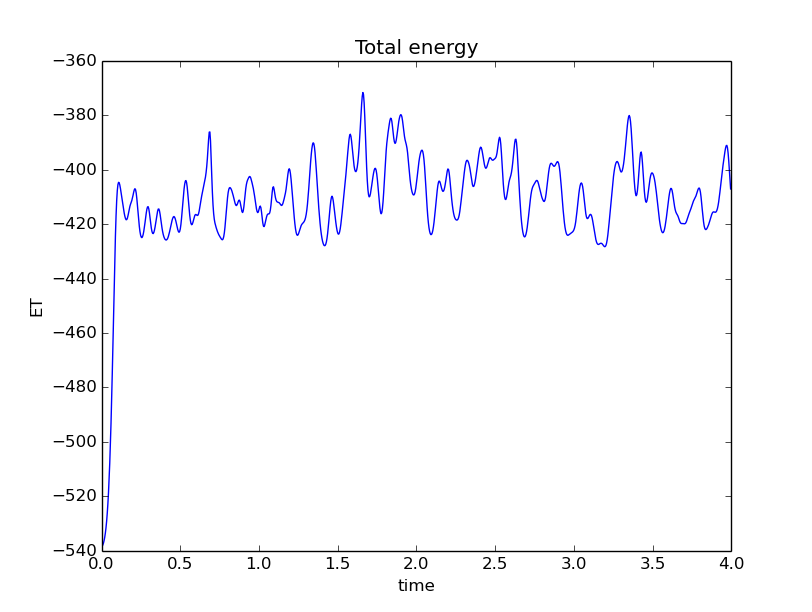
\includegraphics[width=0.7\linewidth]{et_1000}
\caption{The jump in the graph is due to initializing the temperature.}
\label{fig:et_1000}
\end{figure}
Figure \ref{fig:et_1000} displays the total energy at 1000 iterations. Remarkable is the initial jump in the energy early in the simulation. The reason for this is the initialization of the temperature. The temperature that is offered as input is not the instantaneous temperature. Rather, it has to be rescaled a number of times with a factor to achieve the desired temperature. This also has an influence on the pressure.
\subsection{Pressure}
\begin{figure}[h]
\centering
\includegraphics[width=0.7\linewidth]{P}
\caption{The pressure as function of the time}
\label{fig:P}
\end{figure}
As a result of temperature initialization , the pressure decreases quickly and oscillations remains fairly constant for the rest of the simulation.
\subsection{Pair correlation function}
\begin{figure}[h!]
        \centering
        \begin{subfigure}[h]{0.45\textwidth}
                \includegraphics[width=\textwidth]{g_0}
                \caption{$t=0$.}
                \label{fig:g_0}
        \end{subfigure}%
        ~ 
        \begin{subfigure}[h]{0.45\textwidth}
                \includegraphics[width=\textwidth]{g_1000}
                \caption{After 1000 iterations.}
                \label{fig:g_1000}
        \end{subfigure}
        ~ 
        \caption{The initial pair correlation distribution and after 1000 iterations.}\label{fig:g}
\end{figure}
Figure \ref{fig:g} shows the results of the pair correlation distribution. Figure \ref{fig:g_0} shows $g$ at $t=0$. At this point the particles are confined to the FCC lattice, so the probability to find a particle at the lattice constant is maximal. After 1000 iteration $g$ evolves. The probability to find a particle close to another, i.e. $r<1.2$ is zero. This is due to the repulsive forces. On the other hand, the probability to find particle far away from another one is also small if not zero. This is caused by the attractive forces.
\subsection{Specific heat}
\begin{figure}[h!]
\centering
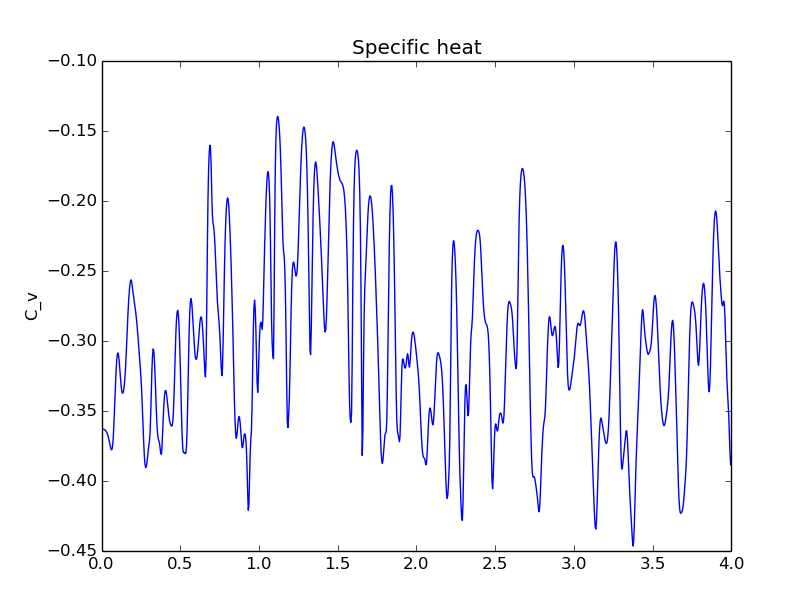
\includegraphics[width=0.7\linewidth]{cv_1000}
\caption{Specific heat with 1000 iterations.}
\label{fig:cv_1000}
\end{figure}
The specific heat also seems to oscillate around a constant value as can be seen in figure \ref{fig:cv_1000}

\section{Conclusion}

In this report the dynamics of argon molecules confined to a finite box was simulated by employing Verlet's algorithm. It was found that the particles still moved quite locally due to interactions, but they weren't restricted to their lattice positions anymore. Quantities such as pressure, correlation function and specific all fluctuate with temperature. If the number of iterations is large enough the oscillations have constant mean. Quantities which can be further investigated are the diffusion constant and statistical errors. 

\section{Appendix}
\definecolor{keywords}{RGB}{255,0,90}
\definecolor{comments}{RGB}{0,0,113}
\definecolor{red}{RGB}{160,0,0}
\definecolor{green}{RGB}{0,150,0}
\lstset{language=Python, 
        basicstyle=\ttfamily\small, 
        keywordstyle=\color{keywords},
        commentstyle=\color{comments},
        stringstyle=\color{red},
        showstringspaces=false,
        identifierstyle=\color{green},
        procnamekeys={def,class},
        frame=single,breaklines=true }

\lstinputlisting{paircorr3D.py} 
\lstinputlisting{Rmatrixfile.py}
\lstinputlisting{cdf.py}
\lstinputlisting{velocitygen.py}
\lstinputlisting[language=fortran,frame=single, breaklines=true]{forcetestken.f95}
\lstinputlisting{update.py}
\lstinputlisting{josplot.py}
\lstinputlisting{MD.py}
\lstinputlisting{CorCalc3d.py}
\lstinputlisting{plots.py}
\end{document}
